\section{Tracking with the Inner Detector} \label{sec:atlas:tracking}

With its closest component, the Insertable B-Layer (IBL)
\cite{Potamianos:2209070}, only 3.3 cm from the interaction point. The Inner
Detector (ID), shown in \cref{fig:inner_detector_diagram}
\cite{ATLAS-TDR-4,ATLAS-TDR-5}, faces the incredible challenge of providing
precise momentum resolution and identification of both primary and secondary
vertex measurements of charged particle tracks all while receiving the highest fluence.

\begin{figure}[!htbp]
  \begin{center}
    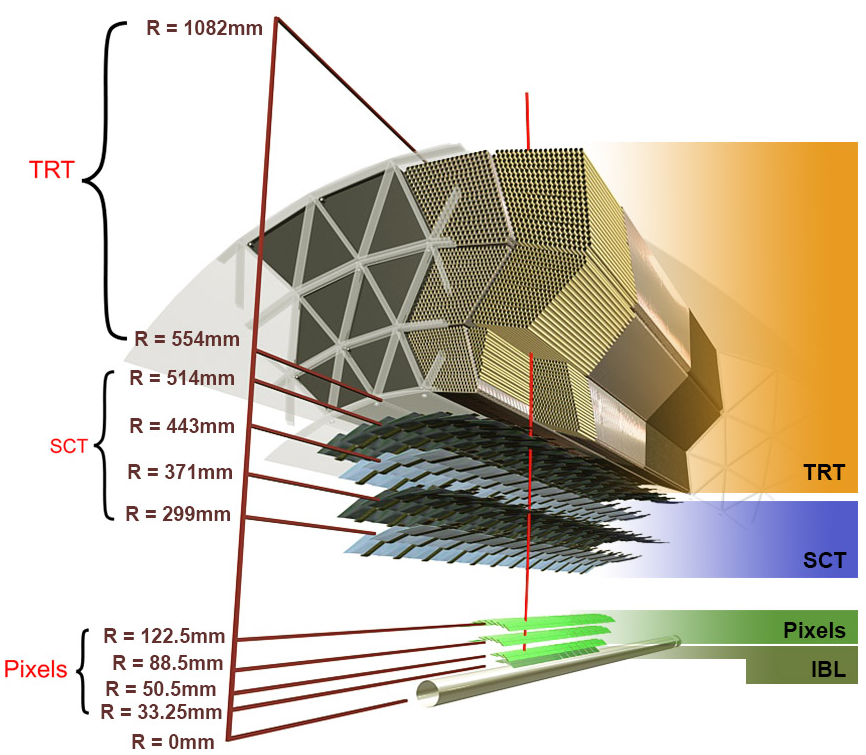
\includegraphics[width=0.8\linewidth]{figures/atlas/inner_detector_diagram}
    \caption{ \cite{Potamianos:2209070} Diagram of inner detector}
    \label{fig:inner_detector_diagram}
  \end{center}
\end{figure}

It is designed to be very compact to reduce the probability of a particle
decaying inside and to give precision measurements of the particles curvature in
the 2T solenoidal magnetic field. This leads to excellent momentum resolution
above the nominal \pT threshold of $0.5$GeV and within the pseudorapidity range
of $|\eta| < 2.5$ as shown in \cref{fig:inner_detector_schematic}.

\begin{figure}[!htbp]
  \begin{center}
    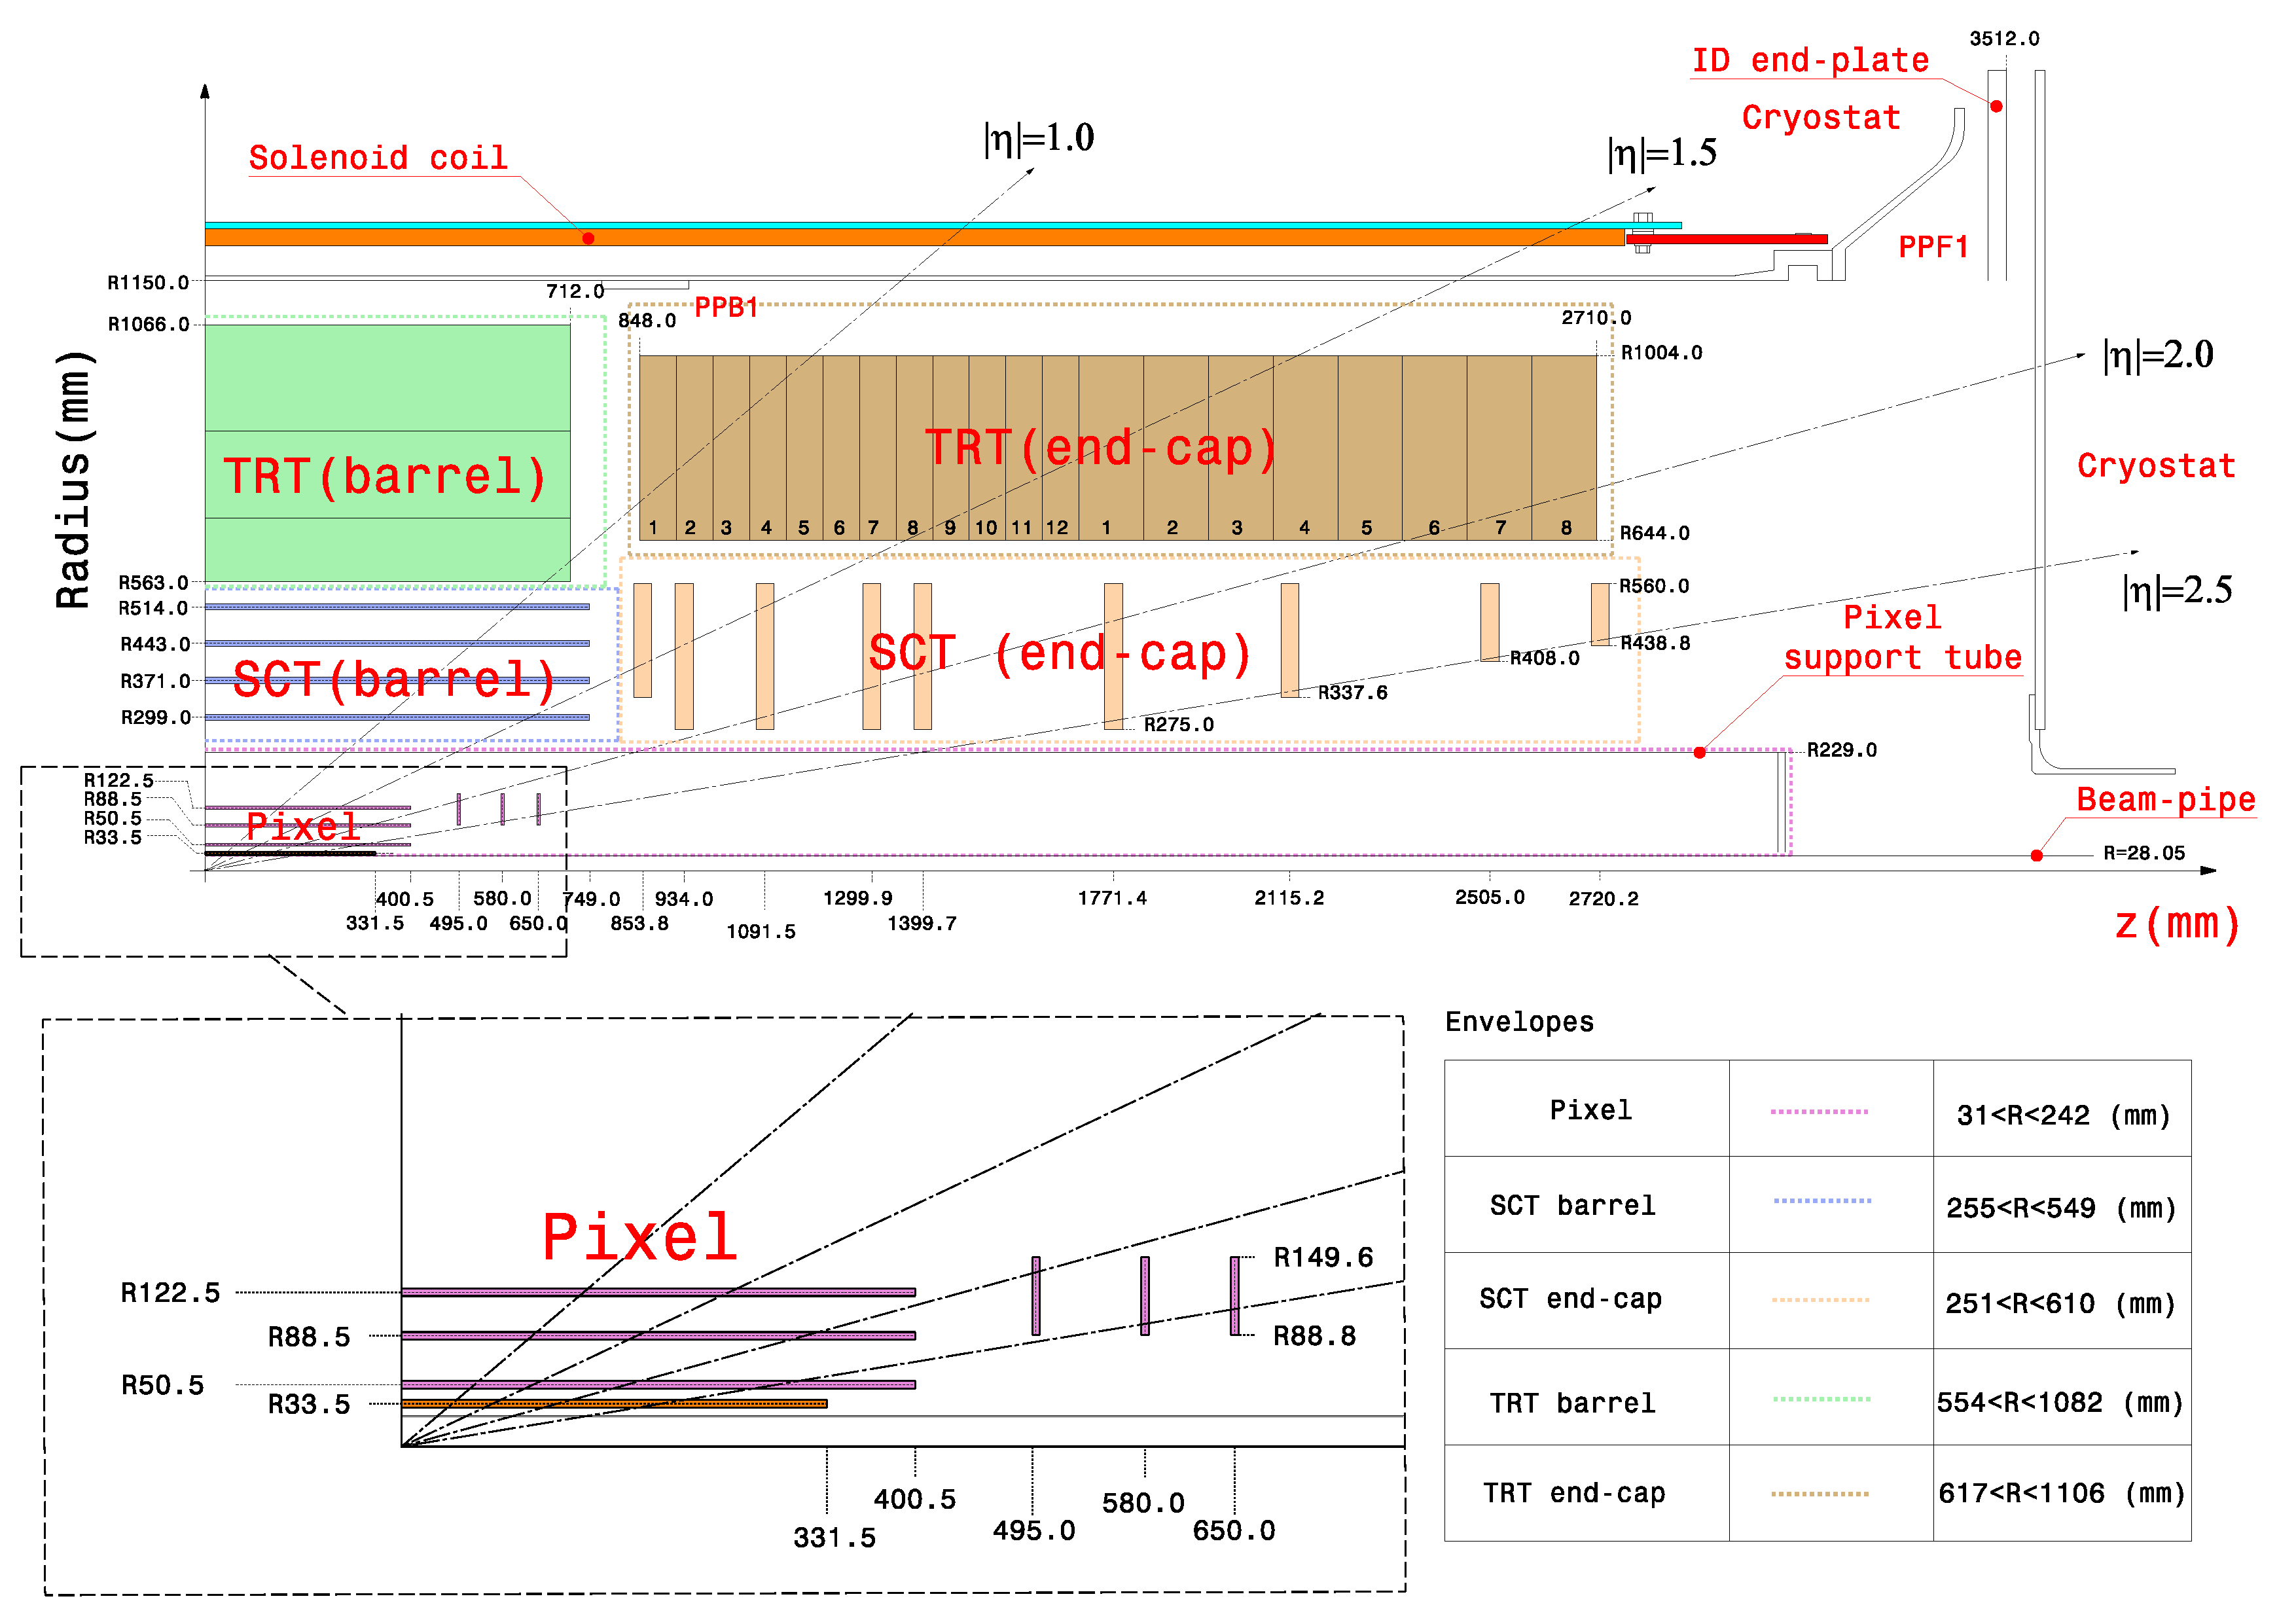
\includegraphics[width=0.8\linewidth]{figures/atlas/inner_detector_schematic}
    \caption{ \cite{PIX-2018-001} Schematic of the Inner Detector including $\eta$
lines.  Each component shown is cylindrically symmetric leading to a
multi-layered detector.}
    \label{fig:inner_detector_schematic}
  \end{center}
\end{figure}

The ID is composed of three different detector technologies for particle
trajector reconstruction: Pixel Detector, Semiconductor Tracker (SCT) and
the Transition Radiation Tracker (TRT).  These will be discussed in the
following sections. 

\subsection{Pixel Detector}

The ATLAS Pixel Detector \cite{PERF-2007-01}, the innermost subdetector of the ID, is designed to
give the best resolution possible as close as possible to the interaction point.
This is accomplished using the 4 barrel layers and 3 disks per endcap as
indicated in \cref{fig:inner_detector_schematic}. The innermost barrel
layer, the IBL, has pixel dimensions of $50\mu $m$(\hat{\phi}) \times 250\mu $m$
(\hat{z}) \times 200\mu $m$(\hat{r})$.  For the other layers the dimensions are
$50\mu $m$(\hat{\phi}) \times 400\mu $m$(\hat{z})$ for about $90\%$ of the pixels
and $50\mu $m$(\hat{\phi}) \times 600\mu $m$(\hat{z})$ for the others, all with a
thickness of $250\mu $m$(\hat{r})$.  This gives a total active area of $1.88 $m$^2$
collected through 92.4 million readout channels, more than half of the total
number of channels for ATLAS. This detailed charged particle information very
close to the interaction point is crucial not only for pattern recognition and
track reconstruction, but also for the reconstruction of the primary and
secondary verticies intrinsic to the decay of $b$-hadrons, a critical element
of the analysis presented in this thesis.

\subsection{Semiconductor Tracker}

Encompassing the Pixel Detector, the Semiconductor Tracker (SCT)
\cite{PERF-2007-01} is composed of double-sided silicon microstrip modules.
Each side of the 4088 modules is constructed out of two silison strip sensors
that are daisy-chained togeather.  The result is 768 composite strips each
$12.6$cm with an inter-strip pitch of $80 \mu$m. In the barrel the strips are
alligned with the $\hat{z}$ direction, while in the end-caps they are aligned
with the $\hat{r}$ direction. In both cases the separation of the strips is
constant in $\hat{\phi}$. The two sides are rotated with respect to each other
by $40 \mu$m to allow for position measurement along the length of the strip.
These modules are then used to tile the 4 barrel layers and 9 disks per endcap
(18 disks in total) as seen in \cref{fig:inner_detector_schematic}.  This
design is chosen to ensure that each charged track interacts with 8 strip
layers (equivalent to four space points).  This information is used to further
measure the momentum and impact parameter, as well as vertex identification of
charged particles.

\subsection{Transition Radiation Tracker}

The Transition Radiation Tracker \cite{PERF-2007-01}, the outermost subdetector
of the ID, provides tracking through the detection of transition radiation from
ultra-relativistic charged particles for $\eta < 2.0$ using 350,000 drift tube
channels also known as straws.  The 4mm diameter straws are filled with a $70\%$
Xe, $27\%$ CO$_2$, and $3\%$ O$_2$ gas mixture and a 31$\mu$m diameter
gold-plated tungsten wire anode at the center for the collection of the
ionization signal. In the barrel 73 azimuthally symetric layers of 144cm straws
are oriented parallel to the beam pipe with an electrical division in the center
of each allowing the two sides to be read out separately.  For each endcap the
straws are radially oriented in 160 symmetric planes each containing 768 37cm
long drift tubes shown in \cref{fig:inner_detector_schematic}.  In both
the barrel and the endcaps polypropylene fibers (barrel) or foils (encaps)
function as the transition radiation material which causes the relativistic
charged particles to radiate and thus ionize the gas in the straw.  The amount
of transition radiation produced is proportional to the Lorentz factor meaning
that lighter particles (e.g. electrons) will produce more radiation.  Thus, by
defining a high and low threshold, we can identify tracks belonging to electrons
by requiring they register more high-threshold hits. There are typically 36 TRT
hits per charged particle track. 
